\documentclass[titlepage]{report}

\usepackage{setspace}

\usepackage[utf8]{inputenc}
\usepackage{amsmath}   
\usepackage{mathtools}
\usepackage{graphicx}
\usepackage{subcaption}
\usepackage{float}
\usepackage{hyperref}
\usepackage{listings}
\usepackage[labelfont=bf]{caption}
\usepackage[margin=3.5cm]{geometry}

\lstset{
	basicstyle=\footnotesize\ttfamily,
}

\title{
\vspace{50pt}\\
\huge \bfseries SKEDGE
\\
\vspace{10pt}
\Large
Smarter course scheduling for our\\
University of Rochester
}

\author{
	Dan Hassin\\
    \vspace{5pt}\\
    Supervised by\\
    Professor Philip Guo\\
    \vspace{2pt}\\
    Department of Computer Science\\
    University of Rochester\\
    Rochester, New York\\
}

\date{April 12, 2016\\
    \vspace{100pt}\\
    submitted in partial fulfillment of\\
    the requirements for the degree\\
    \emph{honors bachelor of science}\\
    \vspace{30pt}\\
    and as an open letter addressed to\\
    the information technology staff\\
    at the university of rochester
    \vspace{-30pt}
}

\begin{document}

\maketitle

%%%%%%%%%%%

\onehalfspacing

\pagenumbering{gobble}
\setcounter{tocdepth}{1}
\tableofcontents

\listoftables

\listoffigures

\clearpage

%%%%%%%%%%%%%%%%%%

\doublespacing

\addcontentsline{toc}{chapter}{Abstract}

\begin{abstract}

\thispagestyle{plain}
\pagenumbering{roman}

In this paper I present Skedge, a web application for students to comfortably and effectively engage with the University's course catalog. Skedge matches and surpasses the capabilities of the existing University tool for this purpose, ``Course Description / Course Schedule'' (CDCS) and presents its information in a more visually appealing way. As a result, Skedge boasts strong user-retention rates, long session durations, and high student adoption despite having virtually no advertisement. Through collected usage data, I demonstrate that \textbf{a)} Skedge's differences from and additions to CDCS are usable and have real-world need, \textbf{b)} the three major use-cases associated with course browsing---direct search, exploratory search, and peer recommendation---are effectively accommodated by Skedge, and \textbf{c)} Skedge's novel search mechanism is user-friendly and self-teaches to users over time.

\end{abstract}


%%%%%%%%%%%%%%%

\pagenumbering{arabic}

\setlength{\skip\footins}{0.75cm}



\chapter{Introduction}

This paper will begin by 

\section{Overview of CDCS}

CDCS is the University's official tool for 

\label{fig:cdcs-index}

\subsection{``Better CDCS''}

%%%

\section{Overview of Skedge}

Skedge is a website I developed in 2014 and have been maintaining and developing since.

Bookmarks

Students, parents, department coordinators, and faculty can all benefit from such tool improvements.

user accounts are lightweight, no login, cookie (browser) based

\ref{fig:sk-index}


\begin{figure}[ht]
    \centering
        \begin{subfigure}[h]{14cm}
            \centering
            \fbox{
                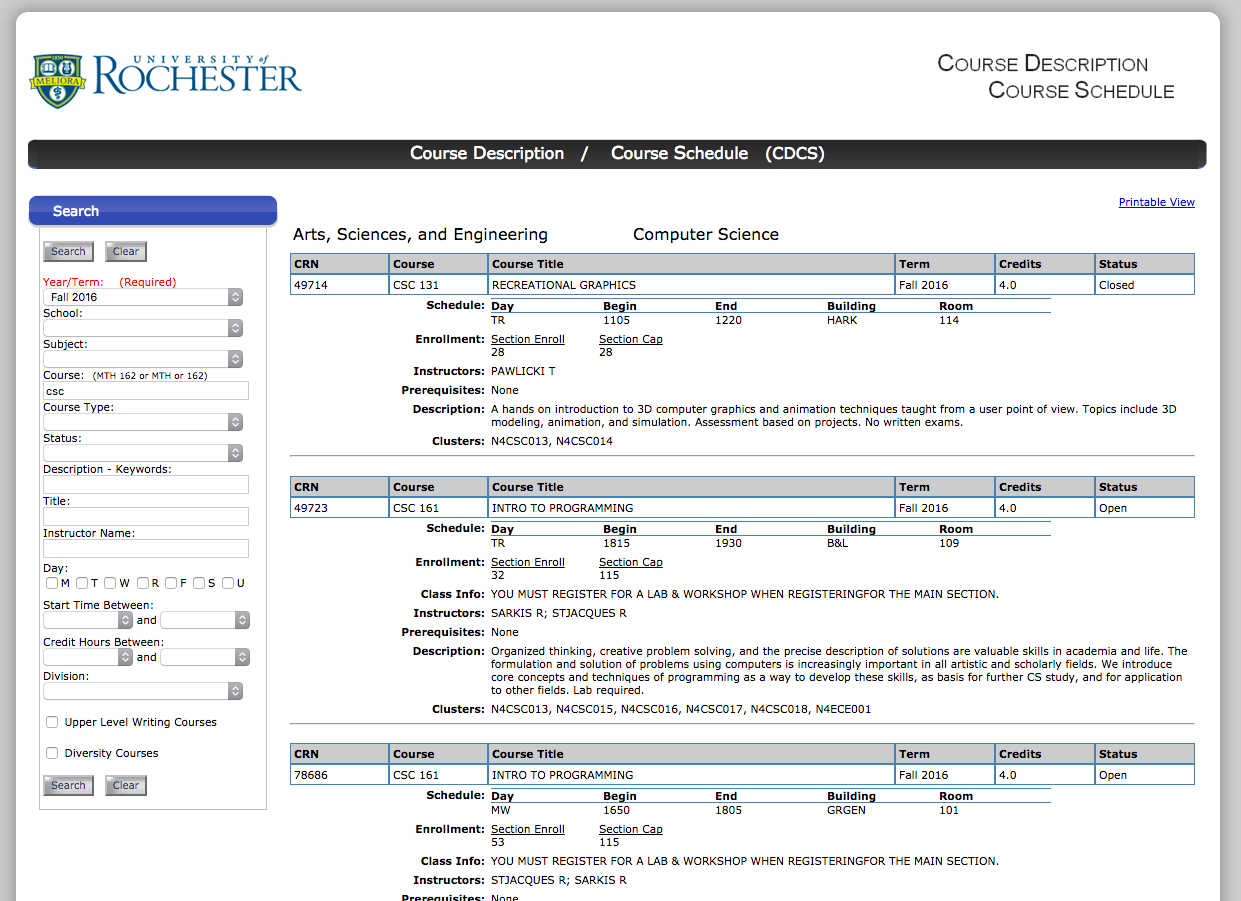
\includegraphics[width=1.00\textwidth]{images/cdcs/index}
            }
            \caption{CDCS, with the search query {\tt csc}}
            \label{fig:cdcs-index}
        \end{subfigure}\\
        \vspace{10pt}\\
        \begin{subfigure}[h]{14cm}
            \centering
            \fbox{
                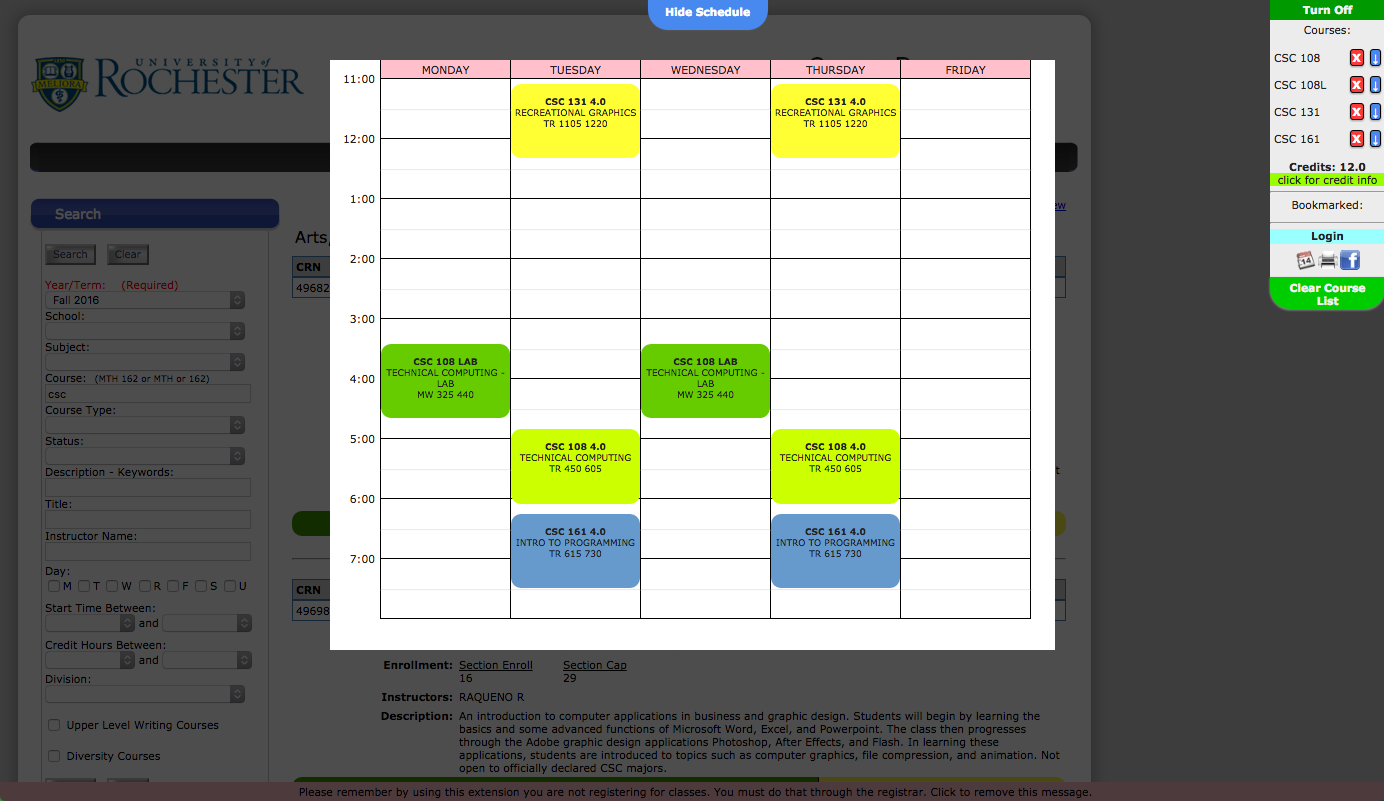
\includegraphics[width=1.00\textwidth]{images/cdcs/better}
            }
            \caption{Better CDCS, a separate browser extension that embeds buttons into the CDCS course results interface, allowing users to add courses to a locally-stored schedule}
            \label{fig:cdcs-better}
        \end{subfigure}
    \caption{CDCS and Better CDCS in their current states}
\end{figure}

\begin{figure}[ht]
    \centering
    \fbox{
        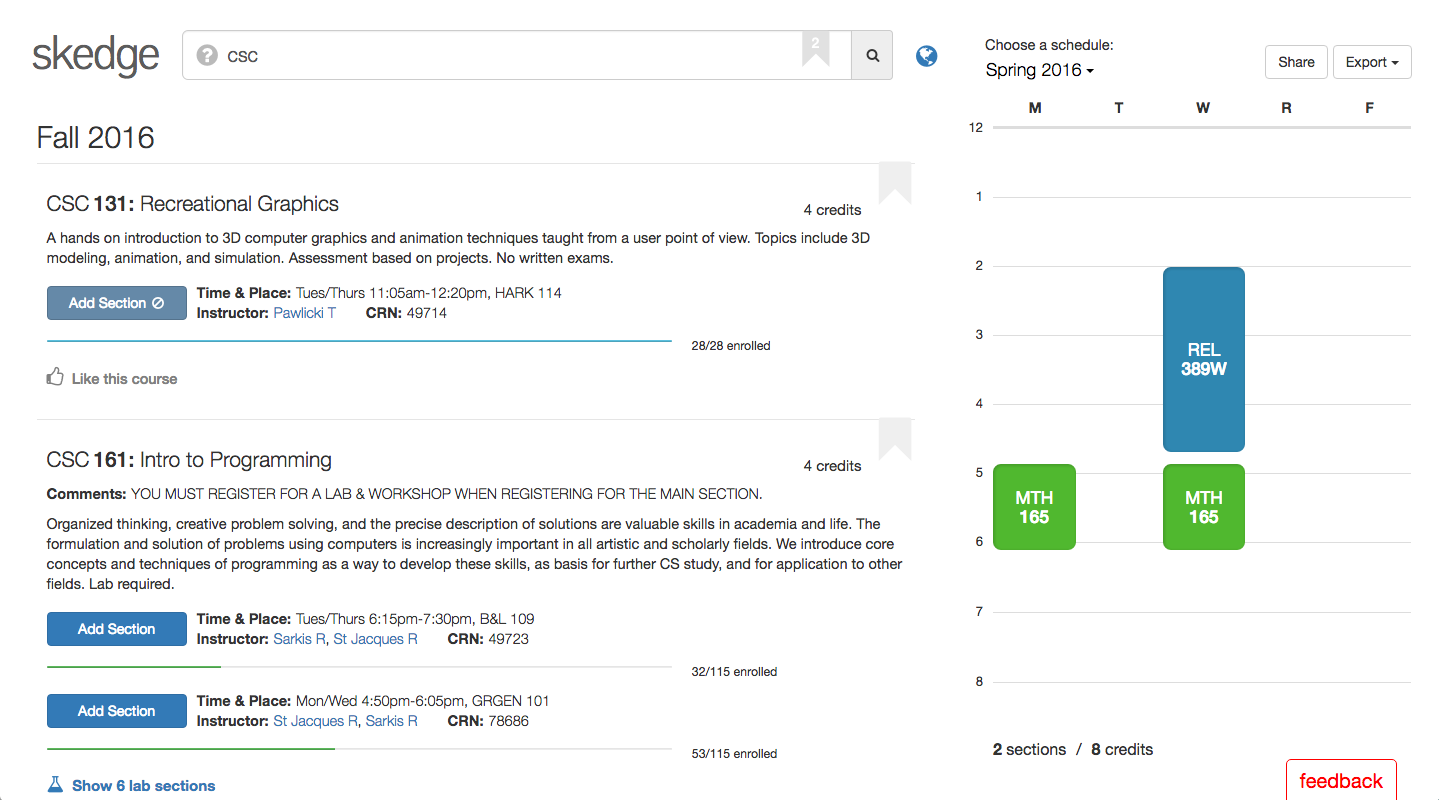
\includegraphics[width=1.00\textwidth]{images/skedge/index}
    }
    \caption[Skedge with the search query {\tt csc}]{Skedge with the search query {\tt csc} and the user's current schedule on the right}
    \label{fig:sk-index}
\end{figure}
\clearpage


\chapter{Design in reaction to CDCS}

From its very inception, Skedge's functionality and visual design were driven by the shortcomings of CDCS. It was built \emph{bottom-up}, not \emph{top-down}---every aspect of the application was either made as a reaction to a particular grievance in CDCS or as the natural evolution of an existing feature. Skedge is thus rooted in \emph{usability} derived from real need, not mere conjecture along the question ``what could students want?''. Its success with students, shown in Chapter 4, demonstrates that this usability extends beyond my own standard and can fulfill the various discovered use-cases of students in general.

In this chapter, I will

%%%

\section{Modernity}

CDCS is an old system, relatively speaking, and its recent development has been stagnant. It launched in 2009, seven years ago, and has hardly changed since. Figure \ref{fig:cdcs2010} shows CDCS in July 2010, which, besides the addition of a few search fields, is identical to its current version. Since its introduction in 2009, we have seen the rise of mobile devices into ubiquity, a boom in ``hacker culture'' and public APIs, and the capability for standalone web applications to be as sophisticated and dynamic as desktop-class applications without the aid of browser extensions.

\begin{figure}[ht]
  \centering
    \fbox{
      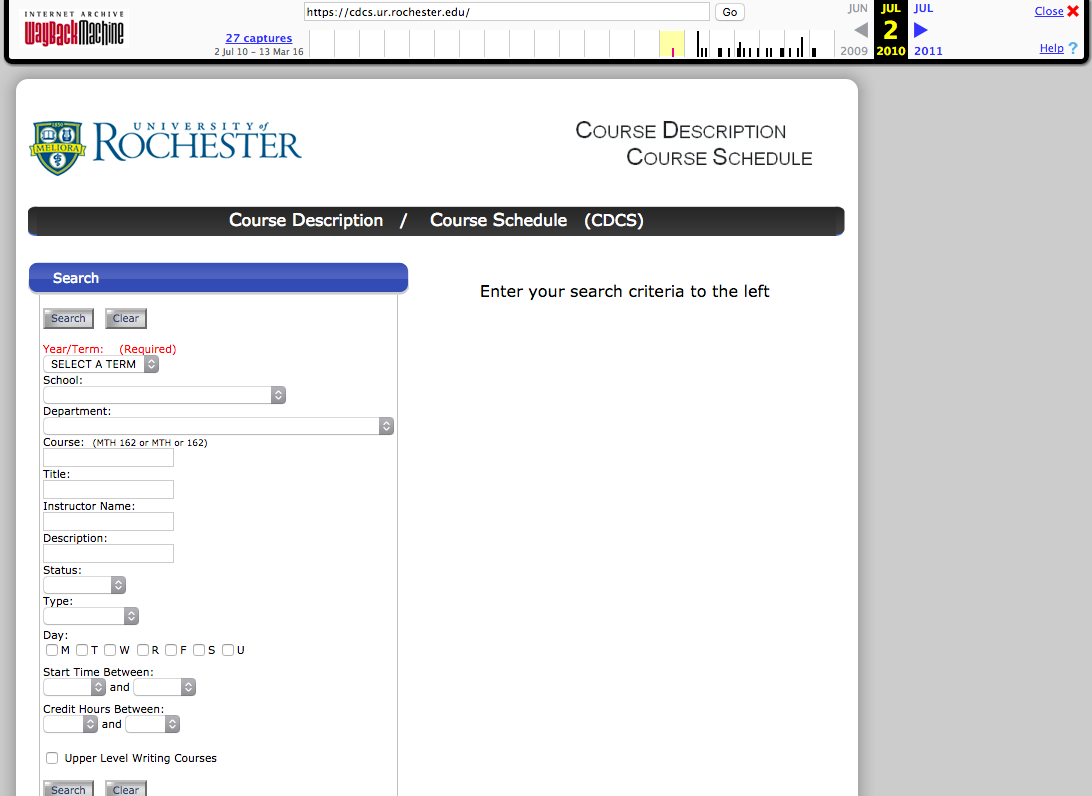
\includegraphics[width=10cm]{images/cdcs/2010}
    }
  \caption{CDCS in July 2, 2010, courtesy of \emph{Archive.org}}
  \label{fig:cdcs2010}
\end{figure}

\subsection{Mobile}

- Important nowadays

- Mobile traffic stat or smth

\begin{figure}[ht]
  \centering
  \begin{tabular}{c c}
    \begin{subfigure}[h]{4cm}
      \centering
      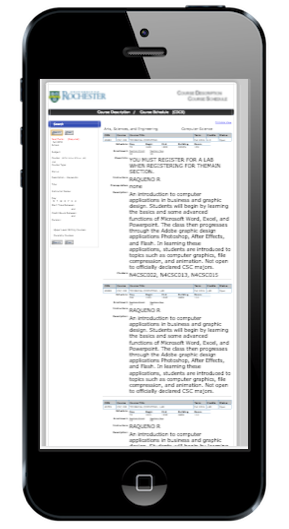
\includegraphics[width=1.00\textwidth]{images/cdcs/mobile}
      \caption{CDCS} \label{fig:cdcs-mobile}
    \end{subfigure}
    \begin{subfigure}[h]{3.9cm}
      \centering
      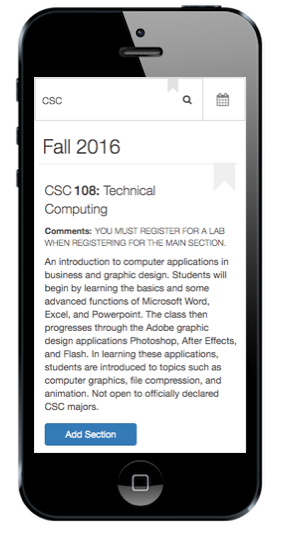
\includegraphics[width=1.00\textwidth]{images/skedge/mobile}
      \caption{Skedge} \label{fig:sk-mobile}
    \end{subfigure}
  \end{tabular}
  \caption{CDCS and Skedge running on a mobile device}
\end{figure}

\subsection{Public API}

With the increasing number of attendees at University of Rochester's hackathons, it is clear that the University's ``hacker culture'' is growing (e.g. more students collaborating to build side-projects that integrate resources and servies often benefitting the student community), and projects that include the University's course catalog are becoming more common. Open-source and open-information services greatly help to foster such innovation, and having public APIs is essential toward this end.

Skedge provides a public JSON API at the root URL \url{http://www.skedgeur.com/api/}, made at the request of a student that was interested in using its course data, and the API has already been used in projects by several other student groups. The endpoints included are \url{/api/courses?q=query} (Skedge's query language---described in detail in section 2.3---is supported here), \url{/api/departments?q=optional_query}, and \url{/api/instructors?q=optional_query}.

\subsection{Built-in scheduler vs. browser extension}

- Better UX

- Data is centralized

\subsection{GET requests vs. AJAX}

- Can use back button

- Can send a link to a course or search

%%%

\section{Usability}

\subsection{Data quality}

- Courses don't shout
- Typos in comments
- 12-hour time

\subsection{Section display}

- Grouped course sections
- Embedded labs (A/B too), workshops, \& recitations

- More concise, space efficient (collapsable)
- Eliminates redundancy of same stuff (instructor, description, course title, etc)
- Don't have to pay more attention that you should to whether it's a different course or the same one

Note that in Figure \ref{fig:cdcs-sections}, the first two boxes are sections for the same course, and the next two are labs for that course. Four more lab sections and \emph{twenty} more workshop sessions for that same course follow below the truncated screenshot. Figure \ref{fig:sk-sections} demonstrates how this information can be conveyed more concisely.

\begin{figure}[ht]
  \centering
  \begin{tabular}{c c}
    \begin{subfigure}[h]{6cm}
      \centering
      \fbox{
        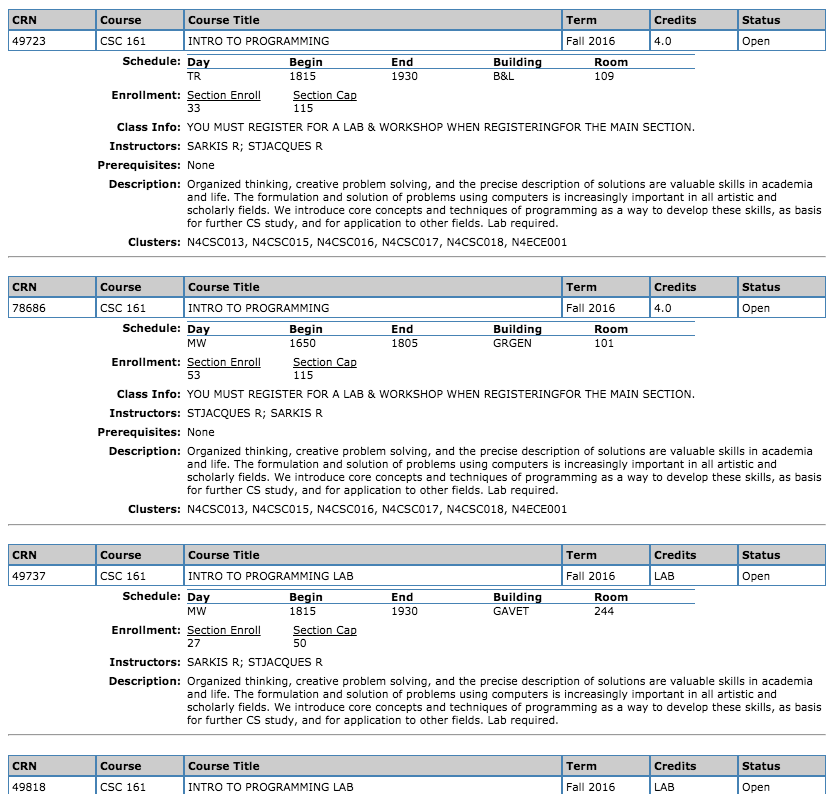
\includegraphics[width=1.00\textwidth]{images/cdcs/sections}
      }
      \caption{Ungrouped sections in CDCS} \label{fig:cdcs-sections}
    \end{subfigure}
    \hspace{15pt}
    \begin{subfigure}[h]{7cm}
      \centering
      \fbox{
        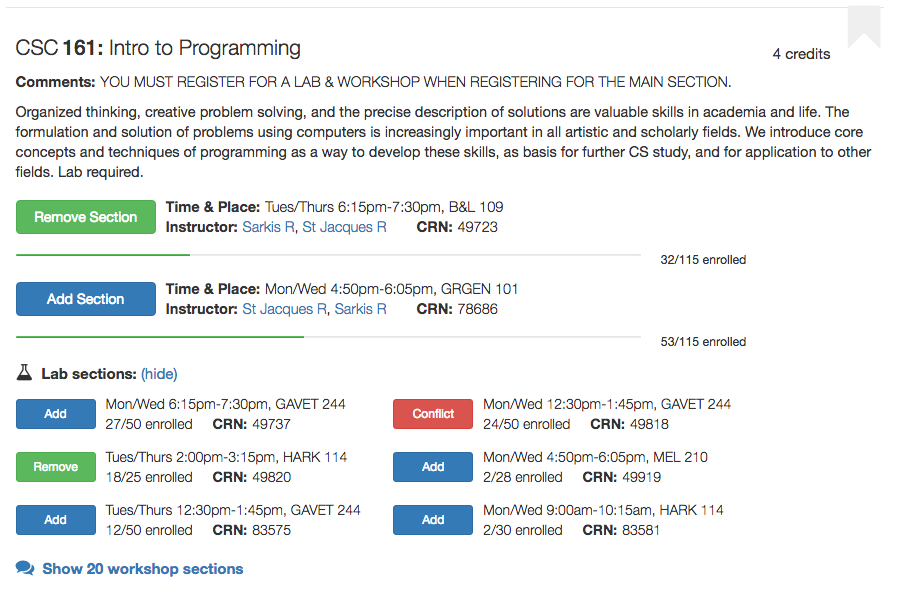
\includegraphics[width=1.00\textwidth]{images/skedge/sections}
      }
      \caption{Grouped sections in Skedge} \label{fig:sk-sections}
    \end{subfigure}
  \end{tabular}
  \caption{Section presentation on CDCS and Skedge}
\end{figure}


\subsection{Course reference}

\begin{figure}[ht]
  \centering
  \fbox{
    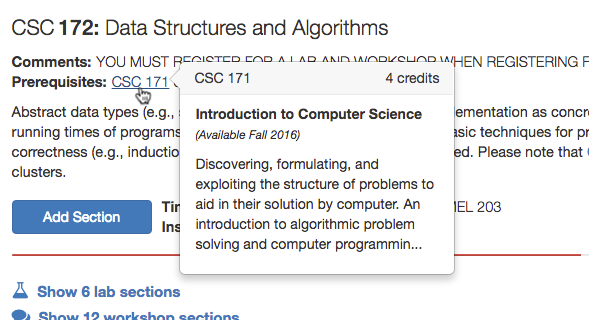
\includegraphics[width=8cm]{images/skedge/hover}
  }
  \caption{Hoverable and clickable course and instructor mentions in Skedge} \label{fig:sk-hover}
\end{figure}

- Clickable/hoverable course links, professor searches

\subsection{Multiple schedule support}

- Old CDCS+betterCDCS system can't keep track of this, have conflicts when adding stuff

\subsection{Exporting to GCal, .ics, image}

- Mobile sync support
- Security: BetterCDCS export gcal is currently broken and sends netID in PLAINTEXT over http(!!!)

\subsection{Search}

Most important usability concern is finding courses.

%%%

\section{Search}

Use cases, natural language.

\subsection{Course selection criteria}

Narrowed it down to three criteria. Keep in mind that \emph{none} of the things listed below are supported by CDCS, and they are all supported by Skedge.

  \subsubsection{Requirements}

  - Finding crosslists
  - Clusters

  \subsubsection{Browsing}

  - ``New'' courses
  - ``Autofit'' search
  - Random
  - Sorts

  \subsubsection{Friends}

  - ``What are my friends taking?'' (``what are you taking this semester'' = probably most common smalltalk phrase uttered on campus)
  - ``What do my friends recommend?'' - ``have you taken this class, and if so, what did you think of it?''

\subsection{Natural language search}

%Figure

See figure.

  \subsubsection{Advantages}

  - 15 fields reduced to 1

  vs form entry:
  - Faster
  - More intuitive
  - More easily extendable

  \subsubsection{Disadvantages}

  Having to know the DSL, grammar ambiguities (can be solved with a `did you mean')

\subsection{Multipurpose}

Used by other links (instructors, course references) around the site

\subsection{Added features}

- CRN (!)
- Crosslist
- Class size

%%%

\section{Social}

\subsection{The issue}

  \subsubsection{Static image vs. live site}

  - Edits don’t update
  - Referencing courses

  \subsubsection{Finding common courses}

  - requires your friends to share their schedules on FB publicly and you to see their post


%%%%%%%%%%%%%%


  - is schedule-first, not search-first
  - typically only occurs for the current semester

%figure

\subsection{Skedge Social}

% Walkthru

  \subsubsection{Friends' course enrollments}

  Mini-feed

  \subsubsection{Friends' course likes}

  \subsubsection{Likes \& enrollments embedded in results}

  \subsubsection{Personal schedule synchronization}

  \subsubsection{Privacy}

  \subsubsection{Notifications}

  %figs of the 2 types
\clearpage


\chapter{Technical overview}

\section{Architecture}

\emph{nginx}, \emph{unicorn}, \emph{Ruby on Rails}, \emph{PostgreSQL}, \emph{React.js}, 

\section{Data storage}

cookies, likes not on fb

\section{Usage data collection}

anonymous, \emph{Ahoy} and Google Analytics.
\clearpage


\chapter{Data analytics}

Hypotheses:

1. Skedge's differences from and additions to CDCS are usable and have real need

2. Skedge’s navigations-per-add and other metrics demonstrate effectiveness of the use cases
a) direct searching, and
b) course browsing

3. Skedge’s DSL is user-friendly; users learn more advanced search types over time by using it

\section{Usage}

\subsection{General}

Since November 3rd 2015 (137 days)
3,768 unique users
4,500 schedules
Average 90 sessions/day
Average 4.92 pages/session
Average 5:31 minutes/session
28\% of sessions are from new users

MOBILE RESULT

\subsection{Search}

% figs

  \subsubsection{Empty searches}

  Can learn from these
  Some funny ones

\subsection{Course blocks}

40\% of sessions have at least one block-click
Average of 4.94 block-clicks per session

\subsection{Social}

90 users have linked Skedge to Facebook
Since March 1st,
4,000+ visits (200 visits/day)
~60\% of visits to /social were returning visitors
90 overlays onto friends’ schedules
10 clicks to Facebook profiles :(
- get stats from the fb dashboard

\subsection{Conclusion}

Success! Considering skedge is OPTIONAL.
+ course blocks (obv usecase, can't click)
+ exports (not supported by thing)
+ mobile

\section{Navigations-per-add}

\subsection{Definitions}

A navigation is defined as
a search, or
a click on an instructor’s name, or
a click on a crosslisted or prerequisite course link

The navigations-per-{add, bookmark} measure is
the number of navigations a user took (within one session) until a course was {added, bookmarked}

\subsection{Trends}

%figs

\subsection{Breaking them apart}

  behavioral patterns
  Direct search for specific course
  Discovery, browsing, exploring

  \subsubsection{Direct searches}

  \subsubsection{Browse}

  % STAT: Find major of users, find how many non-major courses they found

\subsection{Conclusion}

%figs

Effective++

\section{Users' search types over time}

\subsection{Definitions}

Points for search by (omits number and dept.):

description
credits
crosslisted
CRN
instructor
title
year
term
‘random’
upper-level writing

“CSC” → 0
“MTH 165” → 0
“taught by hema” → 1   ✓    (2 searches) 
“random mur 1-2 credits” → 2   ✓    (1 search) 


\subsection{Trends}

% fig

First increase (60.5% of users)
Median: 2 searches
Average: 4.23 searches
(Starting at 1 counts as an increase value of 0)

Second increase (7.9% of users)
Median: 8 searches
Average: 17.52 searches

\subsection{Conclusion}

DSL++
\clearpage


\chapter{Conclusions}

\section{Proposal to the University}

\section{Acknowledgments}

\section{Resources}

\subsection*{Source code}

The source code for Skedge is available online under an open source license:\\
\url{https://github.com/RocHack/skedge}.

\subsection*{Live site}

\noindent The site can be found at: \url{http://skedgeur.com}.
\clearpage

\begin{thebibliography}{1}

	\bibitem{kpcb} Meeker, Mary (2015). http://www.slideshare.net/kleinerperkins/internet-trends-v1

    \bibitem{caps} Wheildon, Colin (1995). \emph{Type and Layout: How Typography and Design Can Get your Message Across - Or Get in the Way.} Berkeley: Strathmoor Press. p. 62. ISBN 0-9624891-5-8.

\end{thebibliography}

\addcontentsline{toc}{chapter}{Bibliography}

\clearpage
\section*{Appendix}

\end{document}
